\section{ПРОЕКТ УЧЕБНО-ЛАБОРАТОРНОГО СТЕНДА}

\subsection{Общая структура стенда и принципы взаимодействия узлов}

Архитектура разрабатываемого учебно-лабораторного стенда построена
по модульному принципу и включает три типа сетевых узлов,
взаимодействующих посредством беспроводного интерфейса Bluetooth.
Такая структура обеспечивает гибкость конфигурации
и позволяет моделировать различные сценарии работы Bluetooth-сетей.

\subsubsection{Типы узлов стенда}

\textbf{Персональный компьютер с USB Bluetooth-адаптером}

Данный узел представляет собой персональный компьютер,
оснащённый внешним USB Bluetooth-адаптером.
Управление осуществляется с использованием операционной системы Linux
и стека BlueZ, что обеспечивает доступ к процедурам обнаружения устройств,
установления соединения и анализа трафика.
Узел данного типа обладает высокой вычислительной мощностью
и удобством конфигурирования.

\textbf{Модуль ESP32 с подключением к ПК}

Узел данного типа реализован на базе микроконтроллера ESP32
и подключается к ПК через USB-интерфейс.
Подключение используется для питания и загрузки прошивки,
в то время как обмен данными осуществляется по радиоканалу Bluetooth.
Такой узел позволяет исследовать поведение встроенных систем
с возможностью оперативной отладки.

\textbf{Автономный модуль ESP32}

Данный узел представляет собой автономное устройство
на базе ESP32 с питанием от аккумулятора.
Он используется для экспериментов, связанных
с изменением расстояния и условий распространения сигнала.
Отсутствие проводного подключения обеспечивает высокую мобильность.

\begin{figure}[H]
\centering
\includegraphics{figures/stand_structure.pdf}
\caption{Общая структура лабораторного стенда}
\label{fig:stand_structure}
\end{figure}

\subsubsection{Принципы взаимодействия узлов}

Взаимодействие между узлами осуществляется
в диапазоне 2{,}4 ГГц по стандарту Bluetooth.
Узлы могут работать в ролях ведущего и ведомого,
что позволяет реализовывать различные топологии.

\begin{enumerate}[nosep]
    \item \textbf{Соединение точка--точка} ---
    взаимодействие между двумя узлами,
    используемое для изучения базовых параметров соединения;

    \item \textbf{Пикосеть} ---
    сеть с одним ведущим устройством
    и несколькими ведомыми,
    синхронизируемыми по общей частотной последовательности;

    \item \textbf{Скаттернет} ---
    объединение нескольких пикосетей через узлы-мосты.
\end{enumerate}


\subsubsection{Программная организация взаимодействия}

На узлах типа А используется стек BlueZ
и утилиты \texttt{bluetoothctl}, \texttt{btmon}, \texttt{hcidump}
для управления соединениями и анализа трафика.

Узлы на базе ESP32 программируются
с использованием Arduino IDE или ESP-IDF.

Обмен данными осуществляется через стандартные профили Bluetooth:
SPP для классического Bluetooth и GATT для BLE.

\subsubsection{Преимущества архитектуры стенда}

\begin{enumerate}[nosep]
    \item гибкость конфигурации
    и возможность быстрой переконфигурации;

    \item возможность сравнительного анализа различных стеков;

    \item масштабируемость системы;

    \item универсальность для проведения исследований и лабораторных работ.
\end{enumerate}

Таким образом, предложенная архитектура обеспечивает
эффективное моделирование Bluetooth-сетей
и проведение лабораторных исследований.

\subsection{Обоснование выбора аппаратной платформы: модули ESP32}

Ключевым элементом автономных и проводных узлов разрабатываемого лабораторного стенда является микроконтроллерный модуль ESP32 производства компании Espressif Systems. Выбор данной аппаратной платформы обусловлен комплексом технических, экономических и методических факторов, обеспечивающих оптимальное соотношение функциональности, стоимости и удобства интеграции в учебно-исследовательский процесс.

\subsubsection{Технические характеристики и архитектура}

Модуль ESP32 построен на базе двухъядерного 32-разрядного микроконтроллера Xtensa® LX6 с тактовой частотой до 240 МГц~\cite{esp32_bt}. Высокая вычислительная мощность позволяет не только управлять процедурами беспроводного обмена данными, но и выполнять локальную обработку сигналов, расчёт статистических метрик (RSSI, SNR) и реализацию сложных алгоритмов управления топологией сети в реальном времени без привлечения внешних вычислительных ресурсов.

Архитектура модуля включает встроенный радиотрансивер, поддерживающий работу в нелицензируемом ISM-диапазоне 2{,}4--2{,}4835 ГГц. Важнейшим преимуществом ESP32 для целей данного стенда является поддержка гибридного режима работы: модуль одновременно совместим со спецификациями классического Bluetooth (BR/EDR) и Bluetooth Low Energy (BLE). Это позволяет исследовать особенности обоих протоколов на единой аппаратной базе, сравнивать их энергоэффективность, скоростные характеристики и механизмы установления соединения.

\begin{figure}[H]
\centering
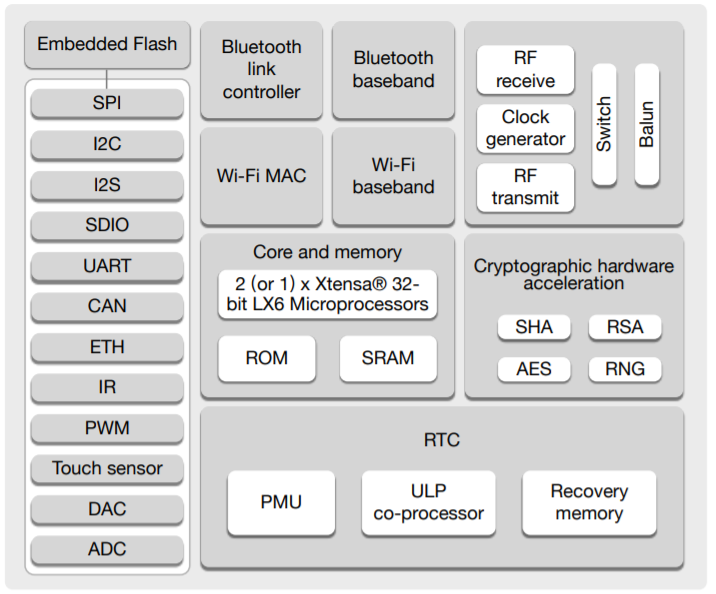
\includegraphics{figures/esp32_block_diagram.png}
\caption{Структурная схема микроконтроллера ESP32}
\label{fig:esp32_block}
\end{figure}

\subsubsection{Интеграция стека протоколов и программная поддержка}

Для реализации логики взаимодействия узлов стенда критически важна доступность развитых средств разработки. ESP32 поддерживает работу с официальным фреймворком ESP-IDF, а также со средой Arduino IDE и платформой PlatformIO. Наличие открытых библиотек (например, \texttt{BluetoothSerial} для классического Bluetooth и \texttt{BLEDevice} для BLE) существенно сокращает время на разработку прошивок узлов.

Программный стек Bluetooth в ESP32 реализует все обязательные уровни ядра системы:
\begin{enumerate}[nosep]
\item \textbf{LMP (Link Manager Protocol)} --- для управления радиосоединением;
\item \textbf{HCI (Host Controller Interface)} --- для взаимодействия между хостом и контроллером;
\item \textbf{L2CAP} --- для мультиплексирования логических каналов и фрагментации пакетов.
\end{enumerate}

Это обеспечивает полную совместимость узлов стенда с внешними USB-адаптерами и другими Bluetooth-устройствами, работающими под управлением стека BlueZ в ОС Linux.

\subsubsection{Энергоэффективность и автономность}

Одним из требований к стенду является мобильность узлов для проведения экспериментов с варьированием расстояния. Модули ESP32 обладают развитыми механизмами энергосбережения, включая режимы глубокого сна (Deep Sleep), в которых потребление тока снижается до нескольких микроампер. Использование компактных литий-полимерных аккумуляторов номинальным напряжением 3{,}7 В и ёмкостью от 500 до 1000 мА·ч обеспечивает автономную работу узлов в течение нескольких часов непрерывного обмена данными.

\subsubsection{Сравнительный анализ альтернатив}

В таблице~\ref{tab:hardware_compare} приведено сравнение модуля ESP32 с другими популярными платформами для Bluetooth-разработки.

\begin{table}[H]
\centering
\caption{Сравнительная характеристика аппаратных платформ для Bluetooth-стенда}
\label{tab:hardware_compare}
\renewcommand{\arraystretch}{1.3}
\begin{tabularx}{\textwidth}{|X|X|X|X|}
\hline
\textbf{Параметр} & \textbf{ESP32} & \textbf{Arduino + HC-05} & \textbf{Nordic nRF52840} \\
\hline
Поддержка BR/EDR и BLE &
Да (Dual-mode) &
Только BR/EDR &
Только BLE \\
\hline
Вычислительная мощность &
Высокая (240 МГц, 2 ядра) &
Низкая (16 МГц) &
Высокая (64 МГц) \\
\hline
Интеграция радиомодуля &
Встроенная &
Внешняя (UART) &
Встроенная \\
\hline
Стоимость модуля &
Низкая (\$3--5) &
Средняя (\$5--8) &
Высокая (\$10--15) \\
\hline
Удобство прототипирования &
Высокое &
Среднее &
Высокое \\
\hline
\end{tabularx}
\end{table}

Как видно из таблицы, ESP32 является единственным решением в низком ценовом сегменте, предоставляющим полноценную поддержку как классического Bluetooth, так и BLE «из коробки». Использование отдельных модулей типа HC-05 ограничивает исследования только профилем SPP и классическим стеком, исключая возможность изучения современных BLE-протоколов (GATT, Advertising). Платформы на базе Nordic Semiconductor, хотя и являются отраслевым стандартом для BLE, имеют более высокую стоимость.

Таким образом, выбор модулей ESP32 в качестве базовой аппаратной платформы узлов стенда является технически и экономически обоснованным решением, полностью закрывающим потребности в исследовании топологий, протоколов и параметров радиоканала технологии Bluetooth.

\subsection{Организация узлов на базе ПК с USB Bluetooth-адаптерами и ESP32}

Архитектура лабораторного стенда предполагает использование гетерогенной структуры, включающей вычислительные узлы на базе персональных компьютеров (ПК) и встраиваемые (embedded) узлы на базе микроконтроллеров ESP32. Такое разделение позволяет гибко комбинировать мощные средства анализа трафика, доступные на ПК, с мобильностью и автономностью микроконтроллерных модулей.

\subsubsection{Узлы на базе ПК с USB Bluetooth-адаптерами}

Персональные компьютеры выступают в роли стационарных или полустационарных узлов стенда, обеспечивая интерфейс управления экспериментами, визуализацию данных и глубокий протокольный анализ. Интеграция ПК в Bluetooth-сеть осуществляется посредством внешних USB Bluetooth-адаптеров.

Выбор внешних адаптеров обусловлен следующими факторами:
\begin{enumerate}[nosep]
    \item \textbf{Универсальность} --- возможность использования стандартных ноутбуков и стационарных ПК без встроенных модулей Bluetooth или с устаревшими версиями стандарта;
    \item \textbf{Гибкость замены} --- быстрая замена адаптера при выходе из строя или необходимости тестирования устройств от разных производителей;
    \item \textbf{Поддержка режима мониторинга} --- многие современные адаптеры на чипах Realtek или CSR поддерживают режим пассивного прослушивания (sniffing), необходимый для перехвата трафика.
\end{enumerate}

Программное обеспечение узлов на базе ПК работает под управлением операционной системы Linux. В качестве основного стека протоколов используется \textbf{BlueZ} --- официальный стек Bluetooth для ядра Linux~\cite{bluez_stack}. BlueZ предоставляет полный набор инструментов для работы с Bluetooth-устройствами, включая утилиты командной строки \texttt{bluetoothctl}, \texttt{hcitool}, \texttt{gatttool} и демон \texttt{bluetoothd}.

Ключевым преимуществом использования Linux и стека BlueZ является наличие интерфейса HCI (Host Controller Interface), который позволяет перенаправлять сырые данные Bluetooth-пакетов в инструменты анализа, такие как Wireshark или btmon. Это реализует сценарий №4 из требований к стенду --- перехват и анализ трафика в реальном времени. ПК может выступать как в роли центрального устройства (Central/Master), инициирующего соединения, так и в роли периферийного (Peripheral/Slave), эмулируя работу датчиков или сервисов.

\subsubsection{Узлы на базе микроконтроллеров ESP32}

Микроконтроллеры ESP32 формируют мобильную часть стенда. В зависимости от способа питания и подключения они разделяются на два подтипа: проводные (подключенные к ПК по USB для отладки) и автономные (питающиеся от Li-Po аккумуляторов).

\textbf{Аппаратная реализация.} Модуль ESP32 интегрирует радиочастотный трансивер, работающий в диапазоне 2,4 ГГц, и поддерживает спецификации Bluetooth v4.2 BR/EDR и BLE. Антенна выполнена в виде печатной дорожки на плате модуля.

\textbf{Программная реализация.} Прошивка узлов разрабатывается в среде Arduino IDE с использованием официальных библиотек Espressif ~\cite{esp_idf_bt_docs} (\texttt{BluetoothSerial} для классического Bluetooth и \texttt{BLEDevice} для BLE). Программный код узлов реализует следующие функции:
\begin{itemize}[nosep]
    \item Инициализация радиомодуля и настройка параметров рекламы (Advertising) или сканирования (Scanning);
    \item Обработка событий подключения и отключения;
    \item Генерация тестовых данных и их передача по профилям SPP или GATT;
    \item Измерение уровня принимаемого сигнала (RSSI) и передача этих данных на управляющий ПК.
\end{itemize}

Для автономных узлов критическим аспектом является управление энергопотреблением. Хотя в базовых лабораторных работах узлы работают в активном режиме, архитектура прошивки предусматривает возможность перевода модуля в режим глубокого сна (Deep Sleep) между циклами передачи данных, что имитирует работу реальных IoT-устройств.
